\chapter{Overview della piattaforma \label{chap:two}}
\fancyhead[RO]{\bfseries Overview della piattaforma}

Come abbiamo detto precedentemente, una città diventa smart grazie all'applicazione di tecnologie che si combinano con l'architettura, gli oggetti che usiamo e perfino il nostro corpo per cercare di risolvere problemi economici, ambientali e sociali. Grazie ad hardware poco costoso come il Raspberry Pi o l'Arduino, si è formato un ecosistema di sensori caratterizzati dal loro costo ridotto e dalla loro semplicità di utilizzo.

Ogni architettura IoT usa sensori e attuatori per raccogliere dati e inviarli nel cloud per processarli. Ad esempio un sensore installato in un contenitore dell'immondizia, misura la quantità di immondizia in modo da gestire al meglio la raccolta in una città; un sensore sulla strada può misurare la velocità del traffico per permettere ai cittadini di evitare strade trafficate.

I numerosi dati provenienti dai sensori sono una vera e propria moneta di scambio nell'economia moderna. Il tema di come gestire queste informazioni ha accelerato la discussione su privacy e sicurezza nel mondo dei big data e quindi in quello dell'IoT.

La piattaforma che ho creato, mette in comunicazione tutti gli attori del sistema: cittadino, comune e attività del territorio; ponendo un focus particolare sulla privacy, in modo che lo scambio di informazione possa avvenire in sicurezza e generare nuove opportunità per il territorio e più in generale per i cittadini.
Ho immaginato un comune che vuole inviare i dati giornalieri di particolato PM10 alla piattaforma e un'attività che li usa per creare servizi al cittadino e generare valore.

\section{Modello di sviluppo}
Per questo progetto è stato utilizzato il modello di sviluppo prototipale. Questo tipo di modello definisce un processo iterativo per il rilascio di versioni del software via via più complete e funzionali. 
Infine ho definito un minimum viable product (MVP) ossia l'insieme minimo di funzionalità che possono essere percepite dal cliente come di valore in una prima versione dell'applicativo.
Le funzionalità principali sono:
\begin{enumerate}
  \item Sicurezza nella trasmissione dei dati
  \item Gestione dell'autorizzazione degli accessi al dato
  \item Visione dei topic accessibili
\end{enumerate}
Questo processo permette di iterare su ogni versione del software grazie a feedback successivi dei clienti senza il rischio di implementare funzionalità non richieste. 

\newpage
\section{Strumenti di sviluppo}
Gli strumenti principali che ho utilizzato per lo svolgimento delle attività di sviluppo del software sono: docker, terminale, sistemi di versioning.
I principali vantaggi, derivanti dall’utilizzo di questi strumenti, sono:
\begin{itemize}
    \item Isolamento
    \item Fast Recovery
    \item Modularità
    \item Sicurezza
\end{itemize}
\subsection{Docker}
\subsection{Git}
\newpage
\section{Protocolli IoT}
Esistono vari protocolli che possono essere usati per lo sviluppo di una piattaforma IoT, molto dipende dall'architettura che si vuole implementare e le funzionalità che si vogliono dare ai clienti finali.
Per questo progetto ho valutato MQTT, CoAP e XMPP.

\subsection{MQTT}
MQTT è un protocollo di comunicazione molto usato in ambito IoT. 
È stato sviluppato per essere usato in sistemi con bassa banda e si basa sul pattern di comunicazione publish/subscribe che richiede un broker per inviare i pacchetti dal publisher al subscribe. In particolare, un publisher, che nel nostro caso è un sensore IoT, invia dati su un "topic" al broker che si occupa di inviare i pacchetti ai client che si sono registrati a quel topic.

Le caratteristiche principali sono:
\begin{itemize}
  \item Il pattern publish/subscribe che permette una distribuzione dei messaggi one-to-many e quindi la possibilità di avere più applicazioni come subscribers.
  \item È utilizzabile qualsiasi payload nel messaggio inviato
  \item Sono implementabili tre tipi di QoS: "Al massimo uno" (<=1) con consegna non assicurata, "Almeno uno" (>=1) in cui la consegna è assicurata ma ci possono essere possibili messaggi duplicati, "Esattamente uno" (=1) che permette la consegna sicura senza duplicati.
  \item Minimo impatto sul traffico nella rete
\end{itemize}

In MQTT i topic sono strutturati come in un file system, ad esempio un publisher potrebbe decidere di pubblicare i dati di un sensore di temperatura su un topic "/home/room1/temperature". In fase si sottoscrizione, si possono utilizzare wildcard, come "+" o "\#", per poter accedere a livelli diversi nella gerarchia definita dal topic; ad esempio iscrivendosi al topic "/home/+/temperature" un subscriber sta richiedendo l'accesso a "home/room1/temperature" ma anche a "/home/room2/temperature".
Il messaggio è composto da 3 parti \cite{MqttStandard}:
\begin{itemize}
    \item \emph{header fisso}. Contiene le informazioni sul tipo di messaggio (publish, subscribe, ecc..) e livello di QoS.
    \item \emph{header variabile} Contiene le informazioni su username, password, last will, ecc.. \cite{MqttIBM}
    \item \emph{payload}.
\end{itemize}

Un'altra caratteristica interessate di questo protocollo, è la possibilità per un client di registrare una sorta di testamento nel caso in cui si disconnetta in modo improvviso. Questi messaggi possono essere utilizzati per avvisare i subscribers di un errore avvenuto nel publisher.

MQTT permette l'implementazione del Last Will and Testament (LWT) per permettere ad un client di essere avvisato quando un publisher chiude la connessione in modo anomalo. Inoltre il publisher puo' specificare se desidera memorizzare un messaggio nel broker, in questo modo, quando un client diventa subscriber di quel topic, riceverà tutti i messaggi memorizzati.

Per quanto riguarda la sicurezza, un broker può richiedere ad un client di autenticarsi mediante username e password; inoltre per garantire la privacy, la comunicazione puo' avvenire in un canale SSL/TLS. 

\newpage
\subsection{CoAP}
CoAP è un protocollo simile all'HTTP. Un client CoAP invia una richiesta verso un server CoAP per richiedere un'azione attraverso la specifica di un metodo. Ogni risorsa è identicata da una URI. Gli scambi di messaggi sono asincroni e vengono scambiati tramite il
protocollo di livello di trasporto UDP.
Esistono 4 tipi di messaggi:
\begin{itemize}
\item Confermable: un messaggio di tipo confermable richiede al server una risposta (Acknowledgement) di avvenuta ricezione.
\item Non-confermable: i messaggi contrassegnati come non-confermable non richiedono l'invio di un acknowledgement; questa tipologia di messaggio è utile per l'invio di pacchetti dai sensori.
\item Acknowledgement: sono le risposte ai messaggi confermable e contengono la risorsa richiesta se disponibile, altrimenti verrà inviato messaggio successivo quando la risorsa sarà disponibile.
\item reset: questa tipologia di messaggio viene inviata dal server quando non riesce a trovare una risposta alla richiesta del client
\end{itemize}
Se il client effettua una richiesta di tipo confermable e il server non ha la risorsa, quest'ultimo risponderà prima con un ACK per evitare che, scaduto il timeout, il client riprovi ad inviare la stessa request, e in seguito, una volta recuperato il dato, invierà una risposta confermable a cui seguirà un ACK del client.

\subsection{XMPP}
XMPP (Extensible Messaging and Presence Protocol) è stato creato originariamente per la messaggistica istantanea (IM).
Il formato dei messaggi scambiati è l'XML. Come l'MQTT, a livello di trasporto utilizza il TCP. Il protocollo può operare seguendo il pattern publish/subscriber.  

XMPP è utilizzato in applicazioni di messaggistica, di chiamate video e addirittura nel gaming. Lo scambio dei dati tramite l'XML rende la comunicazione facilmente estendibile, infatti ci sono più di 200 estensioni registrate con l'XMPP Standards Foundation.

Le connessioni client/server di XMPP sono bidirezionali e ogni parte può inviare dati all'altra fintantocchè il canale è aperto. Questa caratteristica permette di ricevere notifiche (push data) quando è presente nuova infomazione.

Per quanto riguarda la sicurezza, la comunicazione avviene tramite TLS e l'autenticazione attraverso il Simple Authentication and Security Layer (SASL).

Le caratteristiche principali sono:
\begin{itemize}
    \item \emph{Decentrato}. L'architettura dell'XMPP è decentrata e chiunque può eseguire il proprio XMPP server senza la necessità di un master centrale.
    \item \emph{Open Standard}.
    \item \emph{Protocollo solido}. L'XMPP è in uso dal 1999 e ne esistono numerose implementazioni.
    \item \emph{Sicurezza}. SASL e TLS.
\end{itemize}

\section{Conclusioni}
Tutti i protocolli descritti possono essere utilizzati per implementare, in maniera diversa, una piattaforma IoT.
\begin{figure}
\begin{center}
 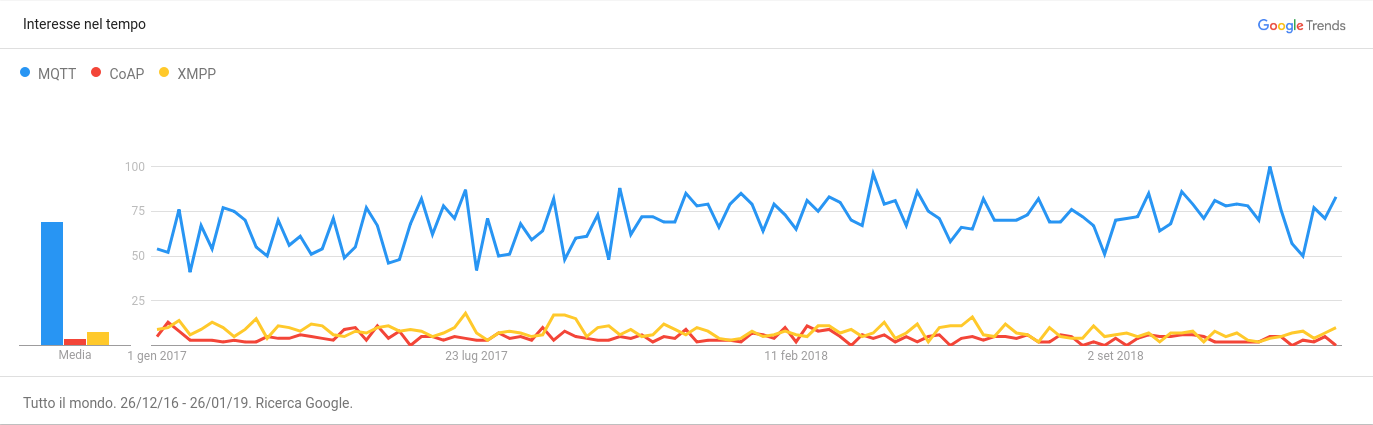
\includegraphics[width=1\textwidth]{trends.png}%
 \caption{Google trends}
 \label{fig:trends}
\end{center}
\end{figure}
Il protocollo che sta avendo maggiormente successo negli ultimi anni, nonostante sia uno dei più recenti, è MQTT: stando agli andamenti di Google Trend (immagine \ref{fig:trends}) l'interesse è almeno 5 volte maggiore di quello del più datato CoAP.

Esistono svariate implementazioni del protocollo MQTT e le numerose librerie open source permettono lo sviluppo di un prototipo in maniera semplice e veloce.

Per questi motivi, ho scelto di implementare una prima versione della piattaforma servendomi di MQTT.
